    \graphicspath{{imagenesFiguras/}} %para que acceda a las fotos en la carpeta directamente

    \subsection{Procedimiento}
    
    Primero que nada, se configuró el generador de señales de manera que produjera una señal senoidal con offset nulo, 20 V de tensión
    pico a pico (es decir 10 V de máxima) y con 1 kHz de frecuencia. Los 20 V pico a pico fue elegidos considerando los 15 V de máxima
    que soportan los cuadripolos, de manera que el valor de la señal fuera lo suficientemente grande como para obtener una buena 
    resolución en el osciloscopio pero a la vez lo suficientemente por debajo de la tensión máxima como para no arriesgar quemar los
    componentes. 
    
    
    Además, ambos cuadripolos poseían una corriente máxima de 50mA. Dada la configuración del generador de ondas, se obtiene que  
    $R_{min} = \frac{10 V}{50 mA} = 200 \Omega$. Para evitar trabajar en valores de corriente muy cercanos al límite, se optó por
    usar una resistencia de 1 $k\Omega$, de manera que $ I = \frac{10 V}{1 k\Omega} = 10 mA $ (muy por debajo de los 50 mA), 
    asegurándonos así de no dañar los equipos. Al mismo tiempo, no se usó una resistencia más grande para evitar trabajar con
    corrientes muy pequeñas, las cuales podrían resultar en mayor ruido en las mediciones. Finalmente, una ventaja adicional de tomar
    ese valor de resistencia es que su amplia diferencia con la resistencia interna del generador de 50 $ \Omega $ (dos órdenes de
    magnitud) implica una menor influencia de la resistencia interna del generador sobre las mediciones, y por lo tanto un comportamiento
    más cercano al ideal.

    \par Dado que resultaba menos trabajoso conectar y desconectar los cuadripolos a la protoboard y entre sí que anular tensiones y
    corrientes, se realizaron las mediciones de manera tal que para cada valor anulado, se medían todos los demás valores con ambos
    cuadripolos y luego con las conexiones para las cuales dichas mediciones fueran útiles, antes de pasar a anular el siguiente valor.
    Por ejemplo, primero se anuló $ I_2 $ y se midieron $ I_1 $, $ V_1 $ y $ V_2 $ para el cuadripolo 9603, luego 
    para el 9609 y luego con ambos conectados en serie y en cascada (nótese que para obtener las ecuaciones de la matriz admitancia, 
    que es la estudiada en el conexionado en paralelo, solo anulan las tensiones $ V_1 $ y $ V_2 $, por lo que realizar las mediciones
    con $ I_2 $ anulada habría sido útil).

    \par Por otra parte, la forma que elegimos de medir corriente usando el osciloscopio fue midiendo la caída de tensión en una 
    resistencia (esto es, la tensión tanto antes como después), y dividiéndola por la impedancia de la misma. Para $ I_1 $ se uso la
    resistencia de $ 1 k\Omega $, y para poder medir la corriente al realizar un cortocircuito en la salida, es decir al anular $ V_2 $,
    se usó una resistencia pequeña de 4,7 $\Omega$ (valor medido con el multímetro). Esta misma introdujo incertezas a las mediciones
    ya que en este caso uno no tendría tensión de salida igual a cero, sino que aproximadamente cero. Aun así se decidió usar este
    método, ya que de otra forma no era posible usar el osciloscopio para medir la corriente y su fase.


    \begin{figure}[H]
        \begin{equation*}
            \begin{tikzpicture}
                \node[shape=rectangle, draw, line width=1pt, minimum width=1.965cm, minimum height=1.965cm] at (5, 2.5){};
                \draw (4.25, 3.25) -| (4.25, 3);
                \draw (4.5, 3.25) -| (4.5, 3);
                \draw (4.75, 3.25) -| (4.75, 3);
                \draw (4, 3.25) to[american resistor, /tikz/circuitikz/bipoles/length=0.840cm] (2.25, 3.25);
                \draw (6.75, 1.75) to[american resistor, /tikz/circuitikz/bipoles/length=0.840cm] (6.75, 3.25);
                \draw (6.75, 3.25) -- (6, 3.25);
                \draw (6.75, 1.75) -- (6, 1.75);
                \node[oscillator, xscale=0.6, yscale=0.6] at (2.544, 2.456){};
                \draw (2.25, 2.75) -- (2.25, 3.25);
                \draw (2.25, 2.162) -- (2.25, 1.75) -- (4, 1.75);
                \node[circ] at (3.75, 3.25){};
                \node[shape=rectangle, minimum width=0.722cm, minimum height=0.472cm] at (1.897, 3.65){} node[anchor=center, align=center, text width=0.5cm, inner sep=5.8pt] at (1.897, 3.65){\scriptsize Ch1};
                \node[shape=rectangle, minimum width=0.722cm, minimum height=0.472cm] at (3.394, 3.65){} node[anchor=center, align=center, text width=0.5cm, inner sep=5.8pt] at (3.394, 3.65){\scriptsize Ch2};
                \node[circ] at (6.75, 3.25){};
                \node[shape=rectangle, minimum width=0.722cm, minimum height=0.472cm] at (6.386, 3.661){} node[anchor=center, align=center, text width=0.5cm, inner sep=5.8pt] at (6.386, 3.661){\scriptsize Ch3};
                \node[sground, xscale=0.6, yscale=0.6] at (2.25, 1.75){};
                \node[shape=rectangle, minimum width=0.722cm, minimum height=0.472cm] at (3.125, 3){} node[anchor=center, align=center, text width=0.5cm, inner sep=5.8pt] at (3.125, 3){\scriptsize 1k};
                \node[shape=rectangle, minimum width=0.722cm, minimum height=0.472cm] at (7.125, 2.5){} node[anchor=center, align=center, text width=0.5cm, inner sep=5.8pt] at (7.125, 2.5){\scriptsize 4,7};
                \node[sground, xscale=0.6, yscale=0.6] at (6.75, 1.75){};
                \draw (2.25, 3.25) -- (2, 3.5);
                \draw (3.75, 3.25) -- (3.5, 3.5);
                \draw (6.75, 3.25) -- (6.5, 3.5);
                \node[circ] at (2.239, 3.239){};
            \end{tikzpicture}
        \end{equation*}
    \caption{Conexionado de los canales del osciloscopio para medir $ V_1, I_1 e I_2 $ en simultáneo con $ V_2 = 0 $.}
    \label{fig: graficoConexionesOsciloscopio}
    \end{figure}

    \begin{figure}[H]
        \centering
        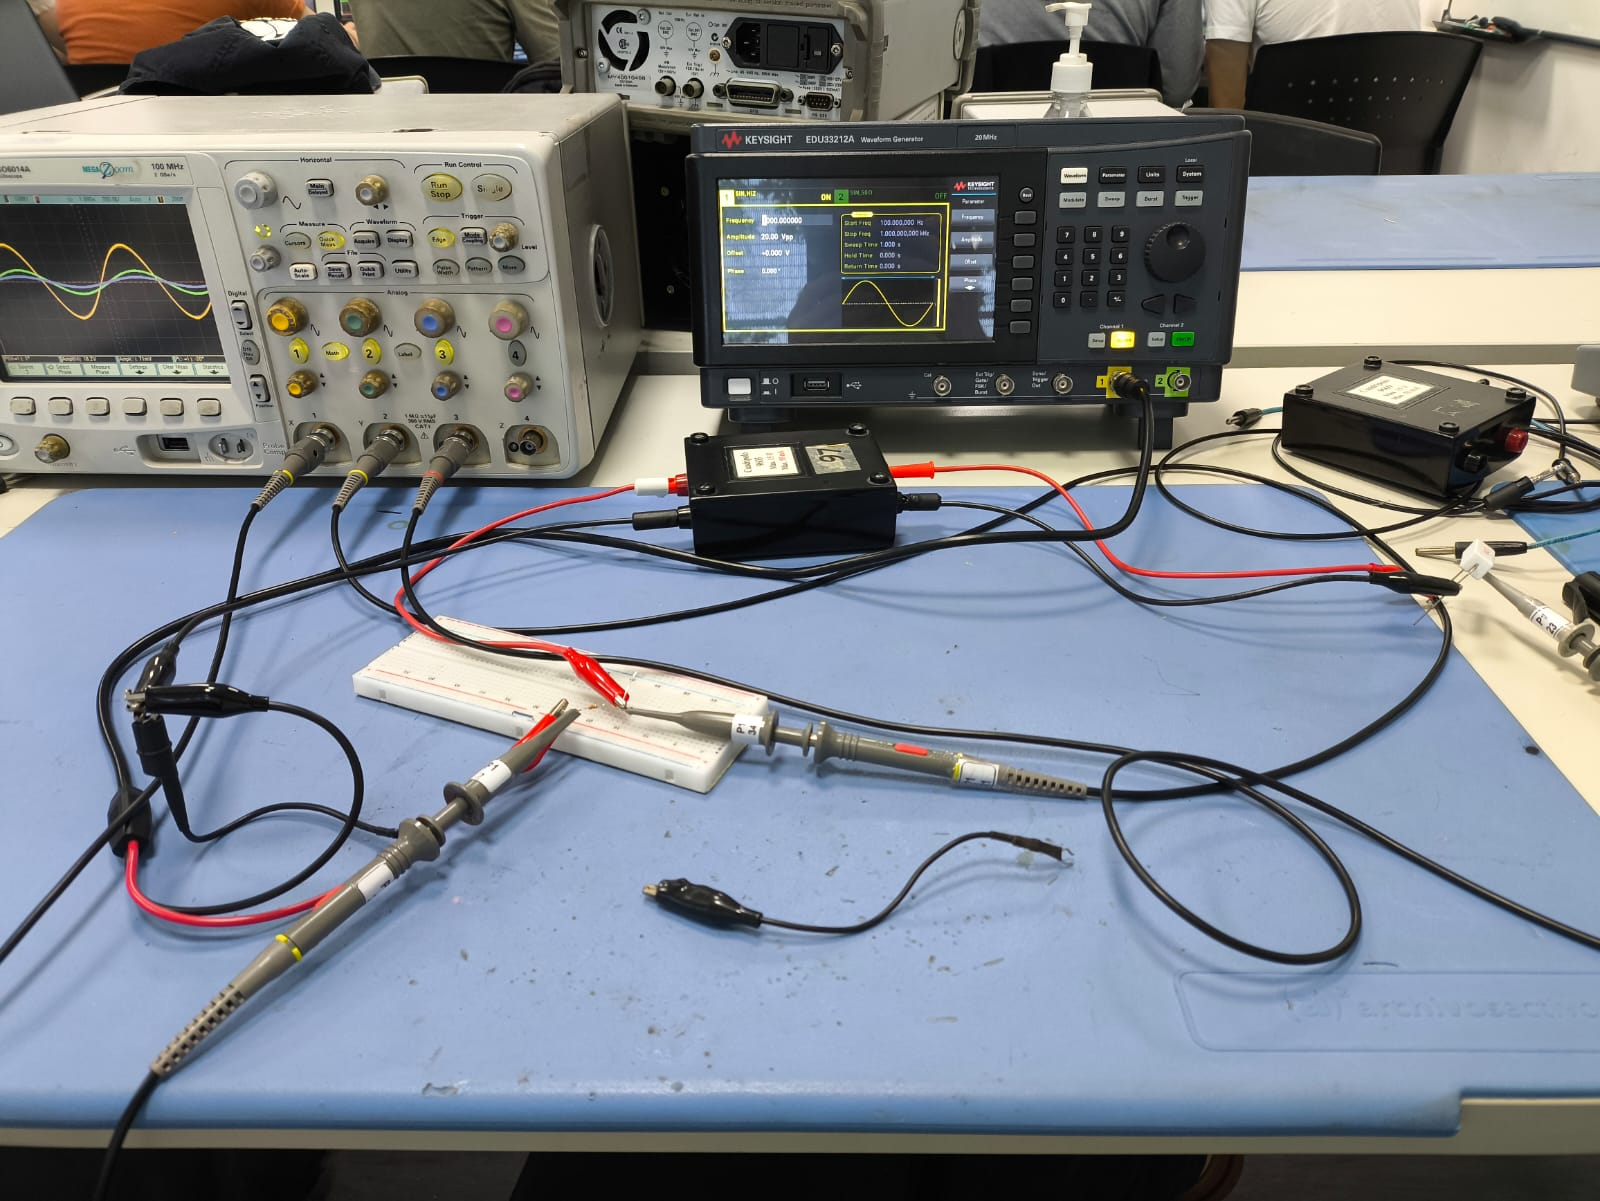
\includegraphics[width=0.5\linewidth]{V2=0.png}
    \caption{Foto de las conexiones para medir $ V_1 $, $ I_1 $ e $ I_2 $ en simultáneo con $ V_2 = 0 $.}
    \label{fig: fotoConexionesOsciloscopio}
    \end{figure}

    \subsection{Datos recolectados}
    
    En el laboratorio se recolectaron los siguientes datos para cada cuadripolo:
    
   \begin{table}[H]
\centering
\begin{tabular}{|l|l|l|l|l|}
\hline
\textbf{9603} & $V_1=0$ & $V_2=0$ & $I_1=0$ & $I_2=0$ \\ \hline 
$V_1$ & $0$ & $0.85\ \mathrm{V}\,\angle\,0^\circ$ & $0.95\ \mathrm{V}\,\angle\,-41^\circ$ & $1.39\ \mathrm{V}\,\angle\,-22^\circ$ \\ \hline
$V_2$ & $0.65\ \mathrm{V}\,\angle\,-24^\circ$ & $0$ & $1.14\ \mathrm{V}\,\angle\,-43^\circ$ & $0.865\ \mathrm{V}\,\angle\,-46^\circ$ \\ \hline
$I_1$ & $5.147\ \mathrm{mA}\,\angle\,-20^\circ$ & $8.5\ \mathrm{mA}\,\angle\,0^\circ$ & $0$ & $8.5\ \mathrm{mA}\,\angle\,4^\circ$ \\ \hline
$I_2$ & $9.1\ \mathrm{mA}\,\angle\,0^\circ$ & $7.941\ \mathrm{mA}\,\angle\,0^\circ$ & $8.6\ \mathrm{mA}\,\angle\,6^\circ$ & $0$ \\ \hline
\end{tabular}
\caption{Mediciones de tensiones y corrientes cuadripolo 9603.}
\label{tab:mediciones9603}
\end{table}

\begin{table}[H]
\centering
\begin{tabular}{|l|l|l|l|l|}
\hline
\textbf{9609} & $V_1=0$ & $V_2=0$ & $I_1=0$ & $I_2=0$ \\ \hline
$V_1$ & $0$ & $1.8\,\mathrm{V}\,\angle\,-16^\circ$ & $1.18\,\mathrm{V}\,\angle\,-58^\circ$ & $1.875\,\mathrm{V}\,\angle\,-30^\circ$ \\ \hline
$V_2$ & $2.5\,\mathrm{V}\,\angle\,-4^\circ$ & $0$ & $2.625\,\mathrm{V}\,\angle\,-17^\circ$ & $1.25\,\mathrm{V}\,\angle\,-58^\circ$ \\ \hline
$I_1$ & $6.617\,\mathrm{mA}\,\angle\,-11^\circ$ & $8\,\mathrm{mA}\,\angle\,4^\circ$ & $0$ & $8\,\mathrm{mA}\,\angle\,7^\circ$ \\ \hline
$I_2$ & $7.3\,\mathrm{mA}\,\angle\,0^\circ$ & $3.676\,\mathrm{mA}\,\angle\,-33^\circ$ & $7.3\,\mathrm{mA}\,\angle\,6^\circ$ & $0$ \\ \hline
\end{tabular}
\caption{Mediciones de tensiones y corrientes cuadripolo 9609.}
\label{tab:mediciones9609}
\end{table}

\begin{table}[H]
\centering
\begin{tabular}{|l|l|l|}
\hline
\textbf{Cascada} & $I_2 = 0$ & $V_2 = 0$ \\ \hline
$V_1$ & $1.2\,\mathrm{V}\,\angle\,-16^\circ$ & $1.22\,\mathrm{V}\,\angle\,-12^\circ$ \\ \hline
$V_2$ & $0.435\,\mathrm{V}\,\angle\,-70^\circ$ & $0$ \\ \hline
$I_1$ & $8.6\,\mathrm{mA}\,\angle\,2^\circ$ & $8.3\,\mathrm{mA}\,\angle\,0^\circ$ \\ \hline
$I_2$ & $0$ & $1.985\,\mathrm{mA}\,\angle\,-12^\circ$ \\ \hline
\end{tabular}
\caption{Mediciones de tensiones y corrientes en conexión en cascada}
\label{tab:corrientes_tensiones_cascada}
\end{table}

\begin{table}[H]
\centering
\begin{tabular}{|l|l|l|}
\hline
\textbf{Serie} & $I_1 = 0$ & $I_2 = 0$ \\ \hline
$V_1$ & $2.34\,\mathrm{V}\,\angle\,-32^\circ$ & $2.64\,\mathrm{V}\,\angle\,-25^\circ$ \\ \hline
$V_2$ & $2.53\,\mathrm{V}\,\angle\,-30^\circ$ & $2.265\,\mathrm{V}\,\angle\,-36^\circ$ \\ \hline
$I_1$ & $0$ & $7.5\,\mathrm{mA}\,\angle\,9^\circ$ \\ \hline
$I_2$ & $7.8\,\mathrm{mA}\,\angle\,11^\circ$ & $0$ \\ \hline
\end{tabular}
\caption{Mediciones de tensiones y corrientes en conexión en serie}
\label{tab:corrientes_tensiones_serie}
\end{table}

\begin{table}[H]
\centering
\begin{tabular}{|l|l|l|}
\hline
\textbf{Paralelo} & $V_1 = 0$ & $V_2 = 0$ \\ \hline
$V_1$ & $0$ & $0.64\,\mathrm{V}\,\angle\,0^\circ$ \\ \hline
$V_2$ & $0.58\,\mathrm{V}\,\angle\,-20^\circ$ & $0$ \\ \hline
$I_1$ & $5\,\mathrm{mA}\,\angle\,-20^\circ$ & $9\,\mathrm{mA}\,\angle\,0^\circ$ \\ \hline
$I_2$ & $8.5\,\mathrm{mA}\,\angle\,0^\circ$ & $5.441\,\mathrm{mA}\,\angle\,-4^\circ$ \\ \hline
\end{tabular}
\caption{Mediciones de tensiones y corrientes en conexión en paralelo}
\label{tab:corrientes_tensiones_paralelo}
\end{table}


     
    \subsection{Cálculos}

	Para el calculo de los parámetros Y, Z y T se usaron las ecuaciones detalladas en el marco teórico. Los resultados obtenidos fueron:
	
	\subsubsection*{Cuadripolo 9603}
	
	\begin{table}[H]
\centering
\begin{minipage}{0.48\textwidth}
\centering
\begin{tabular}{|l|l|}
\hline
\multicolumn{2}{|c|}{\textbf{Matriz de parámetros $Y$}} \\ \hline
$10\,\mathrm{mS}$ & $(7.9 + 0.5523j)\,\mathrm{mS}$ \\ \hline
$9.342\,\mathrm{mS}$ & $(12.789 + 5.694j)\,\mathrm{mS}$ \\ \hline
\end{tabular}
\caption{Matriz de parámetros $Y$ correspondiente al cuadripolo 9603. Matriz calculada a partir de parámetros medidos.}
\label{tab:matriz_Y9603}
\end{minipage}
\hfill
\begin{minipage}{0.48\textwidth}
\centering
\begin{tabular}{|l|l|}
\hline
\multicolumn{2}{|c|}{\textbf{Matriz de parámetros $T$}} \\ \hline
$1.468$ & $-107.04\,\Omega$ \\ \hline
$6.316\times10^{-3}\,\mathrm{S}$ & $-1.07$ \\ \hline
\end{tabular}
\caption{Matriz de parámetros $T$ correspondiente al cuadripolo 9603. Matriz calculada a partir de parámetros medidos.}
\label{tab:matriz_T9603}
\end{minipage}
\end{table}

\begin{table}[H]
\centering
\begin{tabular}{|l|l|}
\hline
\multicolumn{2}{|c|}{\textbf{Matriz de parámetros $Z$}} \\ \hline
$(146.98 - 71.69j)\,\Omega$ & $(75.33 - 80.79j)\,\Omega$ \\ \hline
$(91.47 - 98.08j)\,\Omega$ & $(86.97 - 100.04j)\,\Omega$ \\ \hline
\end{tabular}
\caption{Matriz de parámetros $Z$ correspondiente al cuadripolo 9603. Matriz calculada a partir de parametros medidos}
\label{tab:matriz_Z9603}
\end{table}

Luego, en base a la tabla \ref{tab:matriz_Z9603} se calcularon los parametros Y y T de forma indirecta.

\begin{table}[H]
\centering
\begin{tabular}{|l|l|}
\hline
\multicolumn{2}{|c|}{\textbf{Matriz de parámetros $Y$ (método indirecto)}} \\ \hline
$(14.55 - 1.572j)\,\mathrm{mS}$ & $(-12.16 + 0.886j)\,\mathrm{mS}$ \\ \hline
$(-14.76 + 1.075j)\,\mathrm{mS}$ & $(17.277 + 5.227j)\,\mathrm{mS}$ \\ \hline
\end{tabular}
\caption{Matriz de parámetros $Y$ obtenida por el método indirecto para el cuadripolo 9603}
\label{tab:matriz_Y9603_indirecta}
\end{table}

\begin{table}[H]
\centering
\begin{tabular}{|l|l|}
\hline
\multicolumn{2}{|c|}{\textbf{Matriz de parámetros $T$ (método indirecto)}} \\ \hline
$(1.138 + 0.437j)$ & $(67.37 + 4.91j)\,\Omega$ \\ \hline
$(0.00509 + 0.00545j)\,\mathrm{S}$ & $(0.9878 - 0.0345j)$ \\ \hline
\end{tabular}
\caption{Matriz de parámetros $T$ obtenida por el método indirecto para el cuadripolo 9603}
\label{tab:matriz_T9603_indirecta}
\end{table}
	
	\subsubsection*{Cuadripolo 9609}
	

\begin{table}[H]
\centering
\begin{minipage}{0.48\textwidth}
\centering
\begin{tabular}{|l|l|}
\hline
\multicolumn{2}{|c|}{\textbf{Matriz de parámetros $Y$}} \\ \hline
$(4.176 + 1.520j)\,\mathrm{mS}$ & $(2.627 - 0.323j)\,\mathrm{mS}$ \\ \hline
$(1.953 - 0.597j)\,\mathrm{mS}$ & $(2.913 + 0.204j)\,\mathrm{mS}$ \\ \hline
\end{tabular}
\caption{Matriz de parámetros $Y$ correspondiente al cuadripolo 9609. Matriz calculada a partir de parámetros medidos.}
\label{tab:matriz_Y_9609}
\end{minipage}
\hfill
\begin{minipage}{0.48\textwidth}
\centering
\begin{tabular}{|l|l|}
\hline
\multicolumn{2}{|c|}{\textbf{Matriz de parámetros $T$}} \\ \hline
$(1.324 + 0.704j)$ & $(-468.21 - 143.15j)\,\Omega$ \\ \hline
$(0.003 + 0.006j)\,\mathrm{S}$ & $(-1.738 - 1.310j)$ \\ \hline
\end{tabular}
\caption{Matriz de parámetros $T$ correspondiente al cuadripolo 9609. Matriz calculada a partir de parámetros medidos.}
\label{tab:matriz_T_9609}
\end{minipage}
\end{table}

\begin{table}[H]
\centering
\begin{tabular}{|l|l|}
\hline
\multicolumn{2}{|c|}{\textbf{Matriz de parámetros $Z$}} \\ \hline
$(187.18 - 141.05j)\,\Omega$ & $(70.86 - 145.28j)\,\Omega$ \\ \hline
$(299.76 - 133.46j)\,\Omega$ & $(331.00 - 140.50j)\,\Omega$ \\ \hline
\end{tabular}
\caption{Matriz de parámetros $Z$ correspondiente al cuadripolo 9609. Matriz calculada a partir de parámetros medidos.}
\label{tab:matriz_Z9609}
\end{table}

Luego, en base a la tabla \ref{tab:matriz_Z9609} se calcularon los parametros Y y T de forma indirecta.
	
	\begin{table}[H]
\centering
\begin{tabular}{|l|l|}
\hline
\multicolumn{2}{|c|}{\textbf{Matriz de parámetros $Y$ (método indirecto)}} \\ \hline
$(7.982 + 0.471j)\,\mathrm{mS}$ & $(-2.847 + 2.194j)\,\mathrm{mS}$ \\ \hline
$(-7.290 - 0.303j)\,\mathrm{mS}$ & $(5.122 - 0.961j)\,\mathrm{mS}$ \\ \hline
\end{tabular}
\caption{Matriz de parámetros $Y$ obtenida por el método indirecto para el cuadripolo 9606}
\label{tab:matriz_Y9606_indirecta}
\end{table}

\begin{table}[H]
\centering
\begin{tabular}{|l|l|}
\hline
\multicolumn{2}{|c|}{\textbf{Matriz de parámetros $T$ (método indirecto)}} \\ \hline
$(0.696 - 0.161j)$ & $(136.935 - 5.688j)\,\Omega$ \\ \hline
$(0.003 + 0.001j)\,\mathrm{S}$ & $(1.096 + 0.019j)$ \\ \hline
\end{tabular}
\caption{Matriz de parámetros $T$ obtenida por el método indirecto para el cuadripolo 9609}
\label{tab:matriz_T9609_indirecta}
\end{table}

	\subsection*{Parametros combinados}
	
\begin{table}[H]
\centering
\begin{tabular}{|l|l|}
\hline
\multicolumn{2}{|c|}{\textbf{Matriz de parámetros $Z$ cuadripolos en serie}} \\ \hline
$(334.16 - 212.74j)\,\Omega$ & $(146.20 - 226.07j)\,\Omega$ \\ \hline
$(391.23 - 231.55j)\,\Omega$ & $(417.97 - 240.55j)\,\Omega$ \\ \hline
\end{tabular}
\caption{Matriz de parámetros $Z$ equivalente correspondiente a la conexión en serie de los cuadripolos 9603 y 9609, calculada a partir de $Z_{9603} + Z_{9609}$.}
\label{tab:matriz_Z_serie_9603_9609}
\end{table}

\begin{table}[H]
\centering
\begin{tabular}{|l|l|}
\hline
\multicolumn{2}{|c|}{\textbf{Matriz de parámetros $Z$ serie a partir de mediciones}} \\ \hline
$(291.82 - 196.84j)\,\Omega$ & $(219.41 - 204.60j)\,\Omega$ \\ \hline
$(213.55 - 213.55j)\,\Omega$ & $(244.80 - 212.80j)\,\Omega$ \\ \hline
\end{tabular}
\caption{Matriz de parámetros $Z$ correspondiente a la conexión en serie directa de los cuadripolos 9603 y 9609, calculada a partir de los valores medidos en el laboratorio.}
\label{tab:matriz_Z_serie_directa}
\end{table}

\begin{table}[H]
\centering
\begin{tabular}{|l|l|}
\hline
\multicolumn{2}{|c|}{\textbf{Matriz de parámetros $T$ equivalente (conexión en cascada)}} \\ \hline
$(1.9448 + 1.2786j)$ & $(-407.76 - 375.99j)\,\Omega$ \\ \hline
$(1.70\times10^{-4} + 8.21\times10^{-3}j)\,\mathrm{S}$ & $(-0.0197 - 3.0269j)$ \\ \hline
\end{tabular}
\caption{Matriz de parámetros $T$ equivalente correspondiente a la conexión en cascada de los cuadripolos 9603 y 9609, calculada mediante la multiplicación $T_{9603} \cdot T_{9609}$ conseguidas mediante los datos directos.}
\label{tab:matriz_T_cascada_procuto}
\end{table}

\begin{table}[H]
\centering
\begin{tabular}{|l|l|}
\hline
\multicolumn{2}{|c|}{\textbf{Matriz de parámetros $T$ a partir de mediciones}} \\ \hline
$(1.6214 + 2.2318j)$ & $(-614.61)\,\Omega$ \\ \hline
$(6.109\times10^{-3} + 0.0188j)\,\mathrm{S}$ & $(-3.9421 - 0.8379j)$ \\ \hline
\end{tabular}
\caption{Matriz de parámetros $T$ correspondiente a la conexión en cascada de los cuadripolos 9603 y 9609, obtenida directamente a partir de los valores medidos en el laboratorio.}
\label{tab:matriz_T_cascada_directa}
\end{table}

\begin{table}[H]
\centering
\begin{tabular}{|l|l|}
\hline
\multicolumn{2}{|c|}{\textbf{Matriz de parámetros $Y$ equivalente ($Y_{9603} + Y_{9609}$)}} \\ \hline
$(0.014176 + 0.001520j)\,\mathrm{S}$ & $(0.010527 + 0.000230j)\,\mathrm{S}$ \\ \hline
$(0.011296 - 0.000598j)\,\mathrm{S}$ & $(0.015703 + 0.005899j)\,\mathrm{S}$ \\ \hline
\end{tabular}
\caption{Matriz de parámetros $Y$ equivalente correspondiente a la conexión en paralelo de los cuadripolos 9603 y 9609, calculada a partir de $Y_{9603} + Y_{9609}$.}
\label{tab:matriz_Y_paralelo_suma}
\end{table}

\begin{table}[H]
\centering
\begin{tabular}{|l|l|}
\hline
\multicolumn{2}{|c|}{\textbf{Matriz de parámetros $Y$ (medición directa)}} \\ \hline
$(0.01406)\,\mathrm{S}$ & $(8.62\times10^{-3})\,\mathrm{S}$ \\ \hline
$(8.481\times10^{-3} - 5.930\times10^{-4}j)\,\mathrm{S}$ & $(0.01377 + 5.012\times10^{-3}j)\,\mathrm{S}$ \\ \hline
\end{tabular}
\caption{Matriz de parámetros $Y$ correspondiente a la conexión en paralelo de los cuadripolos 9603 y 9609, obtenida directamente a partir de los valores medidos en el laboratorio.}
\label{tab:matriz_Y_paralelo_directa}
\end{table}

\begin{table}[H]
\centering
\begin{tabular}{|l|l|}
\hline
\multicolumn{2}{|c|}{\textbf{Matriz de parámetros $Y$ equivalente ($Y$ a partir de $Z$)}} \\ \hline
$(0.02253 - 0.00110j)\,\mathrm{S}$ & $(-0.01501 + 0.00381j)\,\mathrm{S}$ \\ \hline
$(-0.02205 + 0.00077j)\,\mathrm{S}$ & $(0.02240 + 0.00427j)\,\mathrm{S}$ \\ \hline
\end{tabular}
\caption{Matriz de parámetros $Y$ equivalente correspondiente a la conexión en paralelo de los cuadripolos 9603 y 9609, calculada a partir de $Z_{9603}$ y $Z_{9609}$.}
\label{tab:matriz_Y_paralelo_desdeZ}
\end{table}

\begin{table}[H]
\centering
\begin{tabular}{|l|l|}
\hline
\multicolumn{2}{|c|}{\textbf{Matriz de parámetros $T$ equivalente ($T_{9603} \cdot T_{9609}$ a partir de $Z$)}} \\ \hline
$(1.0439 + 0.2184j)$ & $(232.09 + 60.03j)\,\Omega$ \\ \hline
$(7.1225\times10^{-3} + 4.298\times10^{-3}j)\,\mathrm{S}$ & $(1.8089 + 0.7745j)$ \\ \hline
\end{tabular}
\caption{Matriz de parámetros $T$ equivalente correspondiente a la conexión en cascada de los cuadripolos 9603 y 9609, calculada a partir de los parámetros $T$ derivados de $Z$.}
\label{tab:matriz_T_cascada_desdeZ}
\end{table}

	
	
	
	
	